% Eigenvalues of the leading k x k corners (k = 1..6, top to bottom) of a random symmetric 6 x 6 matrix:
% each row interlaces the next (Cauchy).
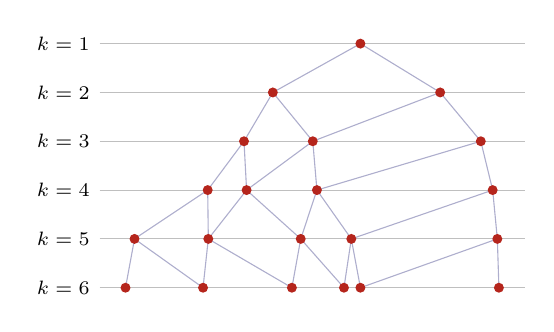
\begin{tikzpicture}[x=1.1cm,y=0.62cm]
\draw[black!25] (-2.978,-1) -- (1.933,-1);
\node[font=\scriptsize,anchor=east] at (-2.978,-1) {$k=1$};
\draw[MidnightBlue!35] (0.034,-1) -- (-0.977,-2);
\draw[MidnightBlue!35] (0.034,-1) -- (0.955,-2);
\draw[black!25] (-2.978,-2) -- (1.933,-2);
\node[font=\scriptsize,anchor=east] at (-2.978,-2) {$k=2$};
\draw[MidnightBlue!35] (-0.977,-2) -- (-1.310,-3);
\draw[MidnightBlue!35] (-0.977,-2) -- (-0.516,-3);
\draw[MidnightBlue!35] (0.955,-2) -- (-0.516,-3);
\draw[MidnightBlue!35] (0.955,-2) -- (1.424,-3);
\draw[black!25] (-2.978,-3) -- (1.933,-3);
\node[font=\scriptsize,anchor=east] at (-2.978,-3) {$k=3$};
\draw[MidnightBlue!35] (-1.310,-3) -- (-1.729,-4);
\draw[MidnightBlue!35] (-1.310,-3) -- (-1.280,-4);
\draw[MidnightBlue!35] (-0.516,-3) -- (-1.280,-4);
\draw[MidnightBlue!35] (-0.516,-3) -- (-0.468,-4);
\draw[MidnightBlue!35] (1.424,-3) -- (-0.468,-4);
\draw[MidnightBlue!35] (1.424,-3) -- (1.561,-4);
\draw[black!25] (-2.978,-4) -- (1.933,-4);
\node[font=\scriptsize,anchor=east] at (-2.978,-4) {$k=4$};
\draw[MidnightBlue!35] (-1.729,-4) -- (-2.574,-5);
\draw[MidnightBlue!35] (-1.729,-4) -- (-1.722,-5);
\draw[MidnightBlue!35] (-1.280,-4) -- (-1.722,-5);
\draw[MidnightBlue!35] (-1.280,-4) -- (-0.655,-5);
\draw[MidnightBlue!35] (-0.468,-4) -- (-0.655,-5);
\draw[MidnightBlue!35] (-0.468,-4) -- (-0.071,-5);
\draw[MidnightBlue!35] (1.561,-4) -- (-0.071,-5);
\draw[MidnightBlue!35] (1.561,-4) -- (1.615,-5);
\draw[black!25] (-2.978,-5) -- (1.933,-5);
\node[font=\scriptsize,anchor=east] at (-2.978,-5) {$k=5$};
\draw[MidnightBlue!35] (-2.574,-5) -- (-2.678,-6);
\draw[MidnightBlue!35] (-2.574,-5) -- (-1.783,-6);
\draw[MidnightBlue!35] (-1.722,-5) -- (-1.783,-6);
\draw[MidnightBlue!35] (-1.722,-5) -- (-0.757,-6);
\draw[MidnightBlue!35] (-0.655,-5) -- (-0.757,-6);
\draw[MidnightBlue!35] (-0.655,-5) -- (-0.156,-6);
\draw[MidnightBlue!35] (-0.071,-5) -- (-0.156,-6);
\draw[MidnightBlue!35] (-0.071,-5) -- (0.034,-6);
\draw[MidnightBlue!35] (1.615,-5) -- (0.034,-6);
\draw[MidnightBlue!35] (1.615,-5) -- (1.633,-6);
\draw[black!25] (-2.978,-6) -- (1.933,-6);
\node[font=\scriptsize,anchor=east] at (-2.978,-6) {$k=6$};
\fill[BrickRed] (0.034,-1) circle (1.8pt);
\fill[BrickRed] (-0.977,-2) circle (1.8pt);
\fill[BrickRed] (0.955,-2) circle (1.8pt);
\fill[BrickRed] (-1.310,-3) circle (1.8pt);
\fill[BrickRed] (-0.516,-3) circle (1.8pt);
\fill[BrickRed] (1.424,-3) circle (1.8pt);
\fill[BrickRed] (-1.729,-4) circle (1.8pt);
\fill[BrickRed] (-1.280,-4) circle (1.8pt);
\fill[BrickRed] (-0.468,-4) circle (1.8pt);
\fill[BrickRed] (1.561,-4) circle (1.8pt);
\fill[BrickRed] (-2.574,-5) circle (1.8pt);
\fill[BrickRed] (-1.722,-5) circle (1.8pt);
\fill[BrickRed] (-0.655,-5) circle (1.8pt);
\fill[BrickRed] (-0.071,-5) circle (1.8pt);
\fill[BrickRed] (1.615,-5) circle (1.8pt);
\fill[BrickRed] (-2.678,-6) circle (1.8pt);
\fill[BrickRed] (-1.783,-6) circle (1.8pt);
\fill[BrickRed] (-0.757,-6) circle (1.8pt);
\fill[BrickRed] (-0.156,-6) circle (1.8pt);
\fill[BrickRed] (0.034,-6) circle (1.8pt);
\fill[BrickRed] (1.633,-6) circle (1.8pt);
\end{tikzpicture}
